\newpage
\section{Ion Temperature Gradient (ITG) Driven Instability}
\label{sec:ITG}

The described electrostatic forces acting on the tokamak plasma cause a variety of collective phenomena. The occurrence of microinstabilities is one of these phenomena. They are instabilities on the spatial scale of the Larmor radius $\rho_\mathrm{L}$ and frequencies much smaller than the cyclotron frequency $\omega_\mathrm{c}$, driven by density and temperature gradients present in the tokamak devices. Turbulence by microinstabilities are considered as one of the main reason for the loss of particle energy and momentum from tokamak plasma \cite{Brizard2007, Garbet2010, Horton1999} which limits the confinement time of tokamak reactors. The most dominant instability in tokamak plasma is the ion temperature gradient (ITG) driven instability. \cite{Coppi1967, Cowley1991, Rudakov1961}

\begin{center}
	\captionsetup{type=figure}
	% \usetikzlibrary{mindmap,backgrounds}
% \usetikzlibrary{decorations.pathmorphing}
% \usetikzlibrary{decorations.markings}
% \usetikzlibrary{arrows.meta,bending}

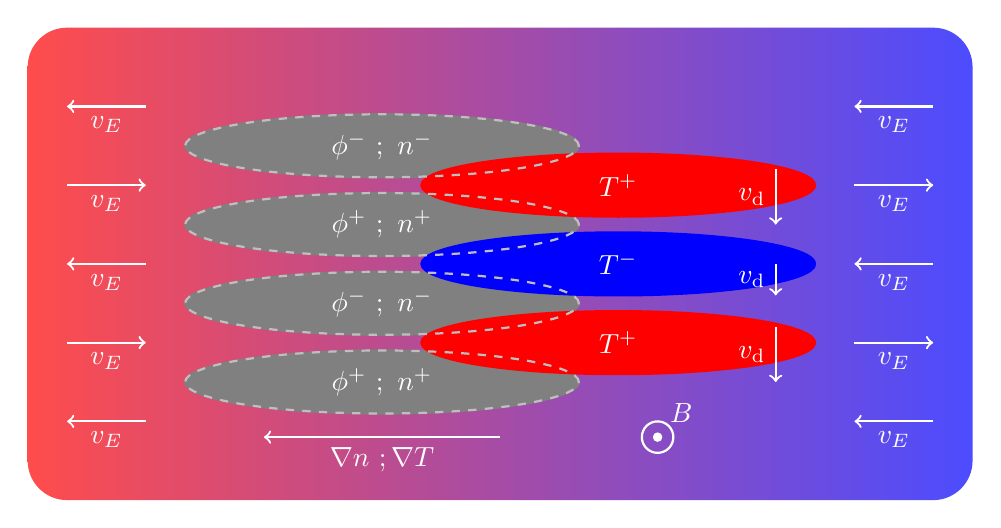
\begin{tikzpicture}
    % Temperature background
    \shade [left color=red, right color= blue, rounded corners = 0.5cm, opacity = 0.7] (0,0) rectangle (12,6);
    % Magnetic field
    \draw [thick, white] (8,0.8) circle (0.2);
    \filldraw [white] (8,0.8) circle (1.5pt);
    \draw (8.3,1.1) node[white]{$\vect{B}$};
    % Density and Potencial cells
    \draw [thick, gray, opacity=1, fill = gray] (4.5,4.5) ellipse (2.5 and 0.4) node[white, opacity=1]{$\phi^{-}~;~n^{-}$};
    \draw [thick, gray, opacity=1, fill = gray] (4.5,3.5) ellipse (2.5 and 0.4) node[white, opacity=1]{$\phi^{+}~;~n^{+}$};
    \draw [thick, gray, opacity=1, fill = gray] (4.5,2.5) ellipse (2.5 and 0.4) node[white, opacity=1]{$\phi^{-}~;~n^{-}$};
    \draw [thick, gray, opacity=1, fill = gray] (4.5,1.5) ellipse (2.5 and 0.4) node[white, opacity=1]{$\phi^{+}~;~n^{+}$};
    % Temperature cells
    \draw [thick, red, opacity=1, fill = red]   (7.5,4) ellipse (2.5 and 0.4) node[white, opacity=1]{$T^{+}$};
    \draw [thick, blue, opacity=1, fill = blue] (7.5,3) ellipse (2.5 and 0.4) node[white, opacity=1]{$T^{-}$};
    \draw [thick, red, opacity=1, fill = red]   (7.5,2) ellipse (2.5 and 0.4) node[white, opacity=1]{$T^{+}$};
    % Temperature and density gradient
    \draw[thick, white, <-] (3,0.8) -- (6,0.8) node[midway, below, white]{$\nabla n~;\nabla T$};
    % Outline Density and Potencial cell
    \draw [thick, lightgray, dashed] (4.5,4.5) ellipse (2.5 and 0.4);
    \draw [thick, lightgray, dashed] (4.5,3.5) ellipse (2.5 and 0.4);
    \draw [thick, lightgray, dashed] (4.5,2.5) ellipse (2.5 and 0.4);
    \draw [thick, lightgray, dashed] (4.5,1.5) ellipse (2.5 and 0.4);
    % Grad B and curvature drift velocity
    \draw[thick, white, ->] (9.5,4.2) -- (9.5,3.5) node[midway, left, white]{$\vect{v}_\mathrm{d}$};
    \draw[thick, white, ->] (9.5,3) -- (9.5,2.6) node[midway, left, white]{$\vect{v}_\mathrm{d}$};
    \draw[thick, white, ->] (9.5,2.2) -- (9.5,1.5) node[midway, left, white]{$\vect{v}_\mathrm{d}$};
    % ExB drift velocity
    \draw[thick, white, <-] (10.5,5) -- (11.5,5) node[midway, below, white]{$\vect{v}_{E}$};
    \draw[thick, white, ->] (10.5,4) -- (11.5,4) node[midway, below, white]{$\vect{v}_{E}$};
    \draw[thick, white, <-] (10.5,3) -- (11.5,3) node[midway, below, white]{$\vect{v}_{E}$};
    \draw[thick, white, ->] (10.5,2) -- (11.5,2) node[midway, below, white]{$\vect{v}_{E}$};
    \draw[thick, white, <-] (10.5,1) -- (11.5,1) node[midway, below, white]{$\vect{v}_{E}$};
    \draw[thick, white, <-] (0.5,5) --   (1.5,5) node[midway, below, white]{$\vect{v}_{E}$};
    \draw[thick, white, ->] (0.5,4) --   (1.5,4) node[midway, below, white]{$\vect{v}_{E}$};
    \draw[thick, white, <-] (0.5,3) --   (1.5,3) node[midway, below, white]{$\vect{v}_{E}$};
    \draw[thick, white, ->] (0.5,2) --   (1.5,2) node[midway, below, white]{$\vect{v}_{E}$};
    \draw[thick, white, <-] (0.5,1) --   (1.5,1) node[midway, below, white]{$\vect{v}_{E}$};
\end{tikzpicture}
	\captionof{figure}{Sketch of ion temperature gradient driven instability on the outboard low field side of the tokamak. \cite{Casson_PHD}}
	\label{fig:ITG}
\end{center}

The ITG-driven instability is present when a sufficiently large ion temperature gradient occurs and is driven by the so-called bad curvature of the outboard low field side of the tokamak. The mechanism is briefly explained with the help of Fig. \ref{fig:ITG} and Ref. \citenum{Beer_PHD, Casson_PHD, Dannert_PHD}. An ion temperature perturbation ($T^\pm \gtrless 0$ \textcolor{blue}{blue} and \textcolor{red}{red} cells) on the outboard low field side of the tokamak causes the modulation of curvature drift and $\nabla B$ drift with velocity $\vect{v}_\mathrm{d}$. The divergence of the velocity $\vect{v}_\mathrm{d}$ is therefore not zero which results in compression of the plasma ($n_\pm \gtrless 0$, \textcolor{gray}{gray} cells). This relates to the perturbation of the potential ($\phi^\pm  \gtrless 0$) in the adiabatic electron response. As stated in the equation for the electric field ($\vect{E} = -\nabla \phi$) the perturbation of the potential $\phi$ causes an electric field $\vect{E}$ which results in a $\exb$ drift with velocity $\vect{v}_E$. The $\exb$ drift direction transports hot plasma in the outer hot region of perturbation ($T^+ > 0$, \textcolor{red}{red} cell) and cooler plasma into inner cold region perturbation ($T^- < 0$, \textcolor{blue}{blue} cell) which reinforce the process and instability grows.
\newpage
The described mechanism causes perturbation on the outboard low field side of the tokamak. This region is also referred to as \enquote{bad curvature} because instability happens there. On the inboard high field side the opposing $\nabla B$ and $\nabla T$ results in a decay of perturbation which is referred to as \enquote{good curvature}. Furthermore, such turbulent structures are called \textit{eddies} which have a typical radial scale of several Larmor radii. \cite{Newins2006}
The initial perturbation is growing if the normalized temperature gradient overcomes a critical value $R/L_{T,\mathrm{c}}$. For nonlinear turbulence with Cyclone Base Case parameters and circular concentric flux-surfaces the critical value is given by $R/L_{T,\mathrm{c}} \sim 6$. \cite{Dimits2000, Isliker2010}